\documentclass[10pt]{article} % For LaTeX2e
\usepackage{tmlr}

\input{math_commands.tex}

\usepackage{hyperref}
\usepackage{url}
\usepackage{booktabs}
\usepackage{graphicx}
\usepackage{tabularx}
\usepackage{amsmath}
\usepackage{amssymb}
\usepackage{xspace}
\usepackage{multirow}

\title{Which Tier, Not Which Peer: Cross-Model Selective Prediction\\from One Cheap Prefill}

% Authors must not appear in the submitted version.
\author{Anonymous Authors}

\newcommand{\scout}{\textsc{scout}\xspace}
\newcommand{\eg}{e.g.\xspace}
\newcommand{\ie}{i.e.\xspace}
\newcommand{\abst}{\bot}

\def\month{09}
\def\year{2026}
\def\openreview{\url{https://openreview.net/forum?id=XXXX}}

% ---------------------------------------------------------------------------------------------
% NUMBERS PENDING (2026-09-18). Text is final; these values will be refreshed from runs in flight:
%  * Table tab:baselines, Fig fig_anchor/fig_savings, the anchor figures in abstract/intro, and the
%    "cap added" 11--25% / 4--12% sentence come from gridmatch/fixedacct, where the two-constraint
%    family's caps were truncated at the expected-cost ceiling (our family stops at 79.6% on LCB).
%    fixedacct2 fixes that; the 78--83.5% losing band should narrow.
%  * Matched point count: our (B,R) family has 12x96 points vs ~96 per baseline. gridmatch/linked
%    runs the linked cap B = k*R (one 96-point sweep), k chosen on calibration by
%    select_linked_k.py. If adopted, Sec. sec:cap and the protocol paragraph change accordingly.
%  * gridmatch/costupd2: same-route cost update across seeds (seed 0: +12..+22% for the price arm).
%  * gridmatch/selc: fixed-C vs calibration-selected-C belief head (+50.6 vs +40.5 at 50%).
%  * Not compiled locally (no TeX on the box); static checks pass (refs, cites, figure paths).
% ---------------------------------------------------------------------------------------------
\begin{document}

\maketitle

\begin{abstract}
Serving a pool of language models under a budget poses a sequential decision for every query:
draw again from the same model, switch to another, or give up.  We show that one forward pass of
the cheapest model over the prompt --- a prefill, with no generated tokens --- carries enough
per-query information to make these decisions well.  Linear probes on the prefill's hidden states
predict each model's success probability and cost for the query, and a one-line rule turns them
into a policy: buy the draw with the largest expected surplus $p_m R - c_m$, and abstain when no
surplus is positive, where $R$ is the dollar value of a correct answer.  On LiveCodeBench the
policy matches gpt-oss-120b's accuracy at 51\% less than calling it on every problem, and 23\%
less than either agreement-gated escalation or the count-based greedy allocation of prior work;
across accuracy targets from 50\% to 75\% it is 11--36\% cheaper than both on every one of five
seeds.  Changing only where the beliefs come from --- same rule, same give-up action, same costs
--- cuts cost at 14 of 14 accuracy targets across LiveCodeBench, TACO and out-of-domain
SWE-bench Verified.  The prefill reads a difficulty shared across models: it tells the policy
whether a problem is worth attempting and which tier of model to try, but not which of several
comparable models suits it, capturing none of 13.5 points of routing headroom on a five-lab pool
of peers.  On LiveCodeBench a give-up action pays only with these per-query beliefs.  The signal transfers to API-only models
at about 25 labels each.  The remaining headroom is belief quality: the probe recovers about half
of the saving perfect beliefs would give at the tightest budgets, and under a tenth near the
pool's ceiling.
\end{abstract}

\section{Introduction}
\label{sec:intro}

An operator serving a pool of language models answers each query by buying draws.  A draw can
come from the model already tried (\emph{resample}), from a different one (\emph{reroute}), or not
at all (\emph{abstain}), and every draw costs money.  \citet{chen2026ror} framed resample-versus-%
reroute as competing uses of a per-query budget; \citet{zhao2026roi} budget a batch of tasks with
a trained skip action; \citet{bouchard2026escalation} treat cascades as a shadow-price problem.
The decision-theoretic machinery is classical \citep{altman1999constrained,weitzman1979optimal}.
What these systems lack is a cheap per-query \emph{belief}: the prior policies condition on
pool-level constants \citep{chen2026ror} or fine-tune the answering model \citep{zhao2026roi}.

We supply the belief from one prefill of the cheapest model in the pool.  Its hidden states,
read before any token is generated, feed two linear heads per model: one predicts the probability
that a fresh draw succeeds on this query, the other the draw's cost.  A policy that is greedy in
the expected surplus $p_mR-c_m$, with abstention as the zero-value action, needs no other
component; sweeping $R$ traces a cost--accuracy frontier.  The probe is trained on 551 labelled
problems, has about 40\,KB of parameters, and costs one 4B-parameter prefill (\$0.00015) per
query.  Only the cheapest model's weights are needed: the other models are observed through
outcomes at training time and a price at decision time.

\paragraph{Findings.}
\begin{itemize}
\item \textbf{Savings against baselines that do not abstain} (Section~\ref{sec:headline}).  On
LiveCodeBench, matching gpt-oss-120b's accuracy (68.0\%) costs \$0.0222 per problem against
\$0.0456 for calling it on everything (Figure~\ref{fig:anchor}); against agreement-gated
escalation and the count-based greedy rule of \citet{chen2026ror} the saving is 11--36\% at
every target from 50\% to 75\%, positive on all five seeds.  On TACO it is 26--50\% at the
35--45\% targets.  The saving is not uniform: there is a band near the pool's ceiling where we
are more expensive (Figure~\ref{fig:savings}).
\item \textbf{The belief source is what pays} (Section~\ref{sec:isolation}).  Holding the rule,
the give-up action and the per-route costs fixed and changing only the beliefs, prefill beliefs
cut cost at matched accuracy at 14 of 14 targets across three pools
(Figure~\ref{fig:isolation}).  Prompt length and TF-IDF features recover little of this; a
learned per-problem decay recovers less than the probe.
\item \textbf{Giving up pays with per-query beliefs} (Section~\ref{sec:mechanism}).  With count
beliefs, every problem looks the same before the first draw: on LiveCodeBench, adding a give-up
action then makes the policy \emph{more} expensive at every target, while with prefill beliefs
it cuts cost by 19\% at the tightest one.  A price-swept policy cannot be run without its
give-up action at all: every price then yields the same policy.
\item \textbf{Which tier, not which peer} (Section~\ref{sec:whethernotwhich}).  The probe reads
a difficulty shared across the pool.  That supports decisions that are monotone in difficulty:
whether to attempt a problem, and which tier of a price-ordered pool to try (with no give-up
action, prefill beliefs still save 7--13\% on LiveCodeBench through the choice of draw alone).
It does not support a choice among comparable models: on a five-lab pool with 13.5 points between
the best model and the pool's oracle, a router on the probe uses one model for 171 of 171 test
problems.
\item \textbf{Transfer and headroom} (Sections~\ref{sec:transfer} and~\ref{sec:diagnostics}).
The probe's ranking of problems transfers to API-only models with no labels, and calibrated
probabilities cost about 25 labels per model.  Perfect beliefs would save 65--75\% at every
target; the probe recovers 54\%, 27\% and 17\% of that at the 50\%, 60\% and 70\% targets.
\end{itemize}

\paragraph{Contributions.}
(i) A budgeted resample/reroute/abstain policy driven by beliefs and costs read from one prefill
of the cheapest model, with the price $R$ as its only parameter (Section~\ref{sec:method}).
(ii) Cost savings at matched accuracy against the baselines a practitioner would deploy ---
agreement-gated escalation, count-based greedy allocation, random allocation, budget-aware
best-of-$K$ and the best fixed plan --- under realised-cost accounting on every arm
(Section~\ref{sec:headline}).  (iii) An attribution of the savings: the belief source isolated on
three pools, its interaction with the give-up action, and the oracle headroom that remains
(Sections~\ref{sec:isolation}--\ref{sec:mechanism}).  (iv) A scope result: the prefill supports
decisions that are monotone in difficulty --- whether to attempt a problem and which tier to try
--- and not a choice among comparable models, and which case applies is visible in measurable
pool structure (Section~\ref{sec:whethernotwhich}).  We claim neither the
MDP nor the Lagrangian relaxation, both classical, nor the observation that hidden states encode
difficulty \citep{llmalreadyknows2025,encodefailures2026,prefillrouter2026}.

\section{Related work}
\label{sec:related}

\paragraph{Sequential and budgeted model selection.}
\citet{chen2026ror} (v1) formalise resample-versus-reroute under a fallible verifier and allocate
a per-query budget greedily by estimated marginal correctness per unit cost, comparing against
single-route, one-commit routing, budget-aware best-of-$K$, cascade and random-allocation
baselines; we reimplement that policy as a baseline.  Version~3 of the same arXiv identifier
\citep{chen2026rorv3} is a different paper under a new title that withdraws the allocation
framework and argues the resample-versus-reroute choice is not identified by the available
evidence; a per-query belief is one way to supply that evidence.  \citet{zhao2026roi} budget a
batch of tasks under a global constraint with a trained solve-or-skip action, by fine-tuning the
answering model.  \citet{bouchard2026escalation} derive Lagrangian switching rules for threshold
cascades.  \citet{seqroute2026} route across the turns of a session under a shared budget with
offline reinforcement learning and a swept multiplier, without resampling or abstention.
\citet{clusterescalate2026} escalate from clusters; \citet{ucci2026} calibrate cascade thresholds
from token margins; \citet{beliefguided2026} treat default-versus-escalate as a POMDP over
response reliability.  Escalating when repeated samples agree or disagree is a common label-free
signal \citep{automix2024,semanticagreement2025}; our agreement-gated baseline belongs to this
family.  None of these estimates a per-query success probability and cost for every model in a
pool from one non-generating forward pass, and none combines resampling, rerouting and abstention
under one price.  \citet{routingsurvey2026} survey routing and cascading; \citet{routinggap2026}
show that part of the router-to-oracle gap is single-draw label noise, which is why our outcome
tensors hold several draws per model.

\paragraph{Prediction from activations.}
\citet{prefillrouter2026} route from prefill hidden states and show that one model's activations
can predict another model's success better than the target's own (encoder--target decoupling);
their router commits once, has no give-up action, and prices cost by median training output
length.  \citet{encodefailures2026} predict a model's own success from its pre-generation
activations; \citet{llmalreadyknows2025} read difficulty from a model's own hidden state and
spend it on adaptive self-consistency; \citet{predictivescheduling2026} allocate a token budget
across a batch from hidden-state predictors.  \citet{scouting2026} feed a repository searcher's
hidden states to a router for coding agents and report that a no-router ablation ties.
\citet{doomed2026} abort agent episodes early with hidden-state probes, and
\citet{quit2026knowing} formalise mid-generation abstention for one model as a reinforcement
learning problem that abstains when the value falls below an abstention reward --- the same
stopping structure as ours, applied within a generation rather than across draws and models.

\paragraph{Difficulty and item response theory.}
Decomposing correctness into item difficulty and model ability is item response theory, with an
active line on language models \citep{jeirt2025,irtnet2025,cmirt2026,adaptivetesting2025}.
\citet{universallatent2026} route zero-shot through a model-independent latent of query
difficulty.  \citet{cofailure2026} bound the gain of any router, vote or cascade by the rate at
which every model fails the same query, and find across 67 models that combining models rarely
beats the best single model without a strong query-level routing signal.  Our ``pool-unsolvable''
fraction is that co-failure rate, and our scope result (Section~\ref{sec:whethernotwhich}) is
consistent with their finding; \citet{routingplateau2026} and \citet{routingcollapse2026}
document routers that learn global trends or collapse onto one model.

\paragraph{Cost and length prediction.}
Response length is linearly decodable from a prompt's hidden state \citep{howmuchleft2026}, and
serving systems predict it for scheduling \citep{trail2024,entropylength2026}.  These predict a
model's own length.  We predict every pool member's cost from one cheap model's prefill and use it
inside the decision rule.  \citet{latencyrouting2026} route on latency as well as cost.

\paragraph{Benchmarks and agents.}
RouterBench \citep{hu2024routerbench} provides an 11-model pool with prices, and its convex hull
of the individual models (the ``Zero Router'') is the right non-adaptive reference;
\citet{llmrouterbench2026} and \citet{agentrouter2026} add further benchmarks.  Stopping or
escalating a single agent's run \citep{agentstop2026,failfast2026,swerouter2026,cope2025} is
adjacent in modality; none prices a multi-model pool or abstains under a budget.

\section{Problem and method}
\label{sec:method}

\subsection{A per-problem MDP}
\label{sec:mdp}

A pool has routes (models) $m\in\{1,\dots,M\}$, each able to produce up to $K_m$ draws for a
problem $x$.  A draw from route $m$ costs $c_m(x)$ in expectation and is verified correct or not;
the episode ends at the first verified success.  Let $n_m$ be the number of failed draws taken
from route $m$ so far and $\mathbf n=(n_1,\dots,n_M)$.  While the problem is unsolved, the
actions are
\[
\mathcal A(\mathbf n)=\{m : n_m<K_m\}\cup\{\abst\}.
\]
Action $m$ pays $c_m(x)$; with probability $p_m(\mathbf n)$ the draw succeeds, the policy
receives $R$ and the episode ends, and otherwise the state moves to $\mathbf n+\mathbf e_m$.
Action $\abst$ (abstain) ends the episode with reward $0$.  Every episode lasts at most
$H=\sum_m K_m$ steps and is undiscounted, so the return is
\[
G \;=\; R\cdot\mathbb 1\{\text{solved}\}\;-\;\text{total cost}.
\]
``Resample'' and ``reroute'' are the two cases of the same action ($n_m>0$ and $n_m=0$).

\paragraph{Beliefs.}
Let $\theta_m(x)$ be the probability that a fresh draw from route $m$ solves $x$.  Give the
problem's per-draw success rate on route $m$ a Beta prior with mean $\theta_m(x)$ and total
pseudo-count $\kappa$.  After $n_m$ failures the posterior predictive probability of success is
\[
p_m(\mathbf n) \;=\; \theta_m(x)\,\frac{\kappa}{\kappa+n_m}.
\]
Routes are treated as independent given $x$, so $\mathbf n$ is a sufficient statistic for the
posterior and the MDP above is the belief MDP of the underlying partially observed problem
\citep{kaelbling1998planning}.  Every optimality statement below is relative to this belief
model.  The independence assumption is weaker than it looks: unconditionally the routes are
strongly coupled (on LiveCodeBench gpt-oss-120b's first-draw success rate is 97.7\% when the
\scout's first draw succeeds and 69.9\% when it fails), but the coupling is problem difficulty,
which $\theta_m(x)$ already encodes; conditioning on the probe's prediction, the \scout's
failure count reduces held-out log-loss only from 0.36886 to 0.36875.

A belief source is a choice of $\theta_m(x)$.  \emph{Count beliefs} set $\theta_m(x)=\bar\theta_m$,
the route's training-set solve rate, identical for every problem; this is the belief model of
\citet{chen2026ror}.  \emph{Prefill beliefs} set $\theta_m(x)$ from the probe
(Section~\ref{sec:probe}).  We fit $\kappa$ by maximum likelihood on the calibration split
separately for each belief source (LiveCodeBench: 0.71 for count beliefs, 0.95 for prefill
beliefs; TACO: 0.40 and 0.66).  The value $\kappa=2$ used by \citet{chen2026ror} loses held-out
log-loss on all six route--dataset cells.

\subsection{The price $R$ and the cost--accuracy frontier}
\label{sec:price}

Over a batch of $N$ problems with an average budget $\bar b$ per problem, the operator wants
\[
\max_{\pi}\;\frac1N\sum_{i=1}^N \Pr_\pi[\text{solved}_i]
\quad\text{s.t.}\quad
\frac1N\sum_{i=1}^N \E_\pi[\text{cost}_i]\;\le\;\bar b .
\]
Relaxing the constraint with a multiplier $\lambda\ge0$ gives a sum of independent per-problem
terms $\Pr[\text{solved}_i]-\lambda\,\E[\text{cost}_i]$; divided by $\lambda$, each is the
expected return $\E[G]$ of Section~\ref{sec:mdp} with $R=1/\lambda$.  The price $R$ is therefore
the dual variable of the budget, read as the dollar value of a correct answer.  A policy that
maximises $\E[G]$ at price $R$ is optimal, under the belief model, among all policies whose
expected spend is no larger than its own: any policy that spent no more and solved more would
have a higher expected return.  Sweeping $R$ therefore traces the frontier.  The achievable set
of (cost, accuracy) pairs is convex, because a policy can randomise between two deterministic
policies problem by problem, and the optimal policy of a constrained MDP is in general such a
mixture \citep{altman1999constrained}.  The frontier of a family of policies is therefore the
upper convex hull of its operating points, and we compare hulls rather than grid points.

\paragraph{Cost at matched accuracy.}
For a family $\mathcal F$, let $C_{\mathcal F}(\alpha)$ be the mean realised cost per problem at
which the hull of $\mathcal F$ reaches overall accuracy $\alpha$ (abstentions count as
failures), by linear interpolation between hull vertices.  The saving of family $\mathcal F$ over
a baseline $\mathcal B$ at target $\alpha$ is
\[
S(\alpha)\;=\;1-\frac{C_{\mathcal F}(\alpha)}{C_{\mathcal B}(\alpha)} ,
\]
defined when both hulls reach $\alpha$.  All costs are \emph{realised}: every arm is charged
what its draws actually cost, and the probe's prefill is charged to every policy that uses it.

\subsection{Decision rule}
\label{sec:rule}

The optimal action values of the MDP satisfy the Bellman optimality equations
\citep{puterman1994markov,sutton2018reinforcement}
\begin{align*}
Q^*(\mathbf n,m) &= -c_m(x)+p_m(\mathbf n)\,R+\bigl(1-p_m(\mathbf n)\bigr)\,V^*(\mathbf n+\mathbf e_m),\\
V^*(\mathbf n) &= \max\Bigl\{0,\;\max_{m\in\mathcal A(\mathbf n)\setminus\{\abst\}} Q^*(\mathbf n,m)\Bigr\},
\end{align*}
with $V^*=0$ once every route is exhausted.  The $0$ is the value of abstaining: the optimal
policy stops exactly when no draw has positive value.

\paragraph{The rule we deploy.}
Let $\pi_\abst$ be the policy that always abstains, so $V^{\pi_\abst}\equiv0$ and its action
values are
\[
Q^{\pi_\abst}(\mathbf n,m)\;=\;p_m(\mathbf n)\,R-c_m(x).
\]
Our policy is greedy with respect to $Q^{\pi_\abst}$:
\[
\pi(\mathbf n)=
\begin{cases}
\abst & \text{if } \max_m Q^{\pi_\abst}(\mathbf n,m)\le 0,\\
\arg\max_m Q^{\pi_\abst}(\mathbf n,m) & \text{otherwise.}
\end{cases}
\]
This is one step of policy improvement from $\pi_\abst$, or equivalently one step of value
iteration from $V_0\equiv0$.  The policy improvement theorem gives $V^\pi\ge V^{\pi_\abst}=0$:
under its own beliefs the policy never expects to lose money at price $R$.  Running $h$ steps of
value iteration from $V_0\equiv0$ gives a depth-$h$ lookahead policy, and $h=H$ recovers $Q^*$
exactly because no episode is longer than $H$.  On our pools $H=18$ and the exact solve visits
342 lattice nodes per decision, so the choice of $h=1$ is empirical, not computational:
deeper lookahead does not reduce cost (Section~\ref{sec:diagnostics}).

\paragraph{The one-step rule stops exactly when the optimal policy does.}
Under the belief model a failure lowers the failed route's belief and leaves the others unchanged,
and a route's cost does not change within an episode, so $Q^{\pi_\abst}(\mathbf n',m)\le
Q^{\pi_\abst}(\mathbf n,m)$ for every state $\mathbf n'$ reachable from $\mathbf n$.  Suppose
$\max_m Q^{\pi_\abst}(\mathbf n,m)\le0$.  Then the same holds at every reachable state, and
backward induction from the exhausted states gives $V^*=0$ at all of them; hence
$Q^*(\mathbf n,m)=Q^{\pi_\abst}(\mathbf n,m)\le0$ for every $m$ and the optimal policy stops at
$\mathbf n$.  Suppose instead that $Q^{\pi_\abst}(\mathbf n,m)>0$ for some $m$.  Since
$V^*\ge0$, $Q^*(\mathbf n,m)\ge Q^{\pi_\abst}(\mathbf n,m)>0$ and the optimal policy continues.
The one-step rule therefore stops in exactly the states where the optimal policy stops --- the
monotone case of optimal stopping \citep{chow1971great} --- and lookahead can change only which
route it tries.  A per-episode cap (Section~\ref{sec:cap}) only removes actions as spend
accumulates and preserves the argument.  The guarantee of Section~\ref{sec:price}, optimality at
the policy's own spend, holds exactly for the depth-$H$ policy; the one-step rule matches it on
when to stop and can differ from it on the order of routes.

\paragraph{Why the rule can stop.}
The count-belief greedy rule of \citet{chen2026ror} ranks routes by the ratio $p_m/c_m$, which is
positive, so it has no stopping condition; its spend is controlled only by a per-episode cap.
The surplus $p_mR-c_m$ changes sign, and abstention needs no threshold or extra head.

\subsection{Beliefs and costs from one prefill}
\label{sec:probe}

Let $\phi(x)\in\R^{d}$ concatenate, at eight layers spanning 25--100\% of the \scout's depth,
the mean over prompt tokens and the last prompt token of the hidden state, computed during the
prompt's prefill with no generation ($d=8\times2\times2560=40{,}960$ for Qwen3-4B).  For each
route $m$:
\[
\hat\theta_m(x)=\operatorname{Platt}_m\!\bigl(\operatorname{logit}^{-1}(w_m^\top\phi(x)+b_m)\bigr),
\qquad
\hat c_m(x)=\rho_m\bigl(a_m+s_m\,\hat T_m(x)\bigr).
\]
The belief head is $L_2$-regularised logistic regression on the success of route $m$'s first
draw, on standardised features with a fixed penalty, followed by Platt scaling fitted on the
calibration split.  Platt scaling can shrink the prediction to a constant, the route's solve
rate, so a useless probe degrades to count beliefs rather than below them.  The cost head
$\hat T_m(x)$ predicts a draw's total tokens by ridge regression, either on log tokens
(exponentiated with Duan's smearing factor \citep{duan1983smearing} so that it estimates a mean)
or on tokens directly, whichever has the higher dollar-space $R^2$ on the calibration split; the
affine recalibration $(a_m,s_m)$ is fitted on the calibration split and likewise falls back to
the route's mean cost when the prediction carries no information.  $\rho_m$ is route $m$'s price
per token.  Every head is fitted on the training split; the test split is used once.  Training
all heads takes 0.16 CPU-seconds.

\subsection{Adding a per-episode cap}
\label{sec:cap}

The price controls spend across problems; a per-episode cap $B$ controls it within one.  With a
cap, action $m$ is admissible only if the realised spend so far plus $\hat c_m(x)$ is at most $B$,
and the rule is otherwise unchanged.  Our method is the family of policies over the grid of
$(B,R)$ pairs; $B=\infty$ is the price-only policy, so the price-only family is contained in it.
The two controls act differently (Section~\ref{sec:mechanism}): the cap bounds how far a single
problem can run, while the price decides which problems are worth starting.

\section{Experimental setup}
\label{sec:setup}

\paragraph{Pools.}
\begin{center}
\small
\begin{tabular}{lcccc}
\toprule
pool & problems & split (train/cal/test) & draws $\times$ routes & role \\
\midrule
LiveCodeBench & 892 & temporal 551/170/171 & $6\times3$ & primary \\
TACO (medium and hard) & 883 & random 547/168/168 & $6\times3$ & primary \\
SWE-bench Verified & 369 & single split & $1\times5$ & out of domain \\
API peers (five labs) & 171 test & calibration split & $1\times5$ & transfer, routing \\
RouterBench \citep{hu2024routerbench} & 36{,}497 & 60\% train & $1\times11$ & routing \\
\bottomrule
\end{tabular}
\end{center}
The three-route pool is Qwen3-4B-Instruct-2507 (the \scout), gpt-oss-20b and gpt-oss-120b, served
with vLLM at a 65{,}536-token cap.  All three sample at temperature 0.2, below the providers'
recommended settings (0.7 for the Qwen model, 1.0 for gpt-oss).  Prices are estimates of
cloud serving cost: \$0.278, \$1.299 and \$11.13 per million tokens, a $40\times$ ratio between
the largest and smallest route.  The \scout prefill costs \$0.000149 per problem on
LiveCodeBench and \$0.000160 on TACO.  Correctness is judged by each benchmark's hidden tests,
and the policy observes that judgement (an oracle verifier; Section~\ref{sec:robust} relaxes
it).  The LiveCodeBench split is temporal: train on contests through September 2024, test on
2025 contests.  The peer pool (deepseek-v4-flash, glm-5, kimi-k2.5, minimax-m2.7, qwen3-max)
comes from five labs via API.  SWE-bench Verified follows \citet{jimenez2024swebench}.

\paragraph{Protocol.}
All policies are compared by replay over stored outcome tensors, so every arm sees identical
draws, outcomes and realised costs.  Draw orderings are resampled per seed: five seeds on
LiveCodeBench and three on TACO; we report mean $\pm$ standard deviation over seeds and the number
of seeds on which the saving is positive.  Baselines are swept over 96 geometrically spaced caps
from one \scout draw to the most expensive realised episode; our method over up to 16 caps on the same
range crossed with 96 prices (12 caps for the results reported here).  Every arm checks its cap against realised spend, and frontiers are
convex hulls (Section~\ref{sec:price}).

\paragraph{Pool structure.}
\label{sec:poolstructure}
\begin{center}
\small
\begin{tabular}{lcccc}
\toprule
pool & best single model & pool oracle & contested & pool-unsolvable \\
\midrule
LiveCodeBench (3 routes) & 69.6\% & 73.1\% & 56.1\% & 26.9\% \\
TACO (3 routes) & 47.6\% & 54.8\% & 35.1\% & 45.2\% \\
SWE-bench Verified (5) & 62.3\% & 71.3\% & 55.0\% & 28.7\% \\
API peers (5 labs) & 71.9\% & 85.4\% & 52.6\% & 14.6\% \\
RouterBench (11) & 84.3\% & 96.1\% & 91.4\% & 3.9\% \\
\bottomrule
\end{tabular}
\end{center}
All columns use one draw per model on the test split.  \emph{Contested} is the share of problems
solved by more than one model and \emph{pool-unsolvable} the share solved by none.  With all six
draws per route, 15.2\% of LiveCodeBench and 41.1\% of TACO test problems remain unsolved.  Pools
with many unsolvable problems reward knowing when to give up; pools with a large gap between the
best model and the oracle reward routing.

\paragraph{Baselines and controls.}
\label{sec:arms}
A \emph{baseline} is a policy a practitioner could deploy instead of ours; none of the baselines
abstains.
\begin{itemize}
\item \textbf{Agreement-gated escalation.}  Start on the cheapest route and resample it; after a
failure, escalate to the next route once two of that route's failed draws produced the same
program (compared after stripping comments, docstrings and whitespace).  Uses no labels.
\item \textbf{Count-belief greedy allocation} \citep{chen2026ror}.  Rank routes by
$\bar\theta_m\kappa/(\kappa+n_m)\,/\,\bar c_m$ and draw until success or until the next draw would
exceed the cap.
\item \textbf{Random allocation.}  Draw from a uniformly chosen affordable route until success or
the cap.
\item \textbf{Budget-aware best-of-$K$.}  Given the cap, pick the route and depth that maximise
the pool-level success probability, and resample that route.
\item \textbf{Fixed-plan hull.}  The convex hull of every fixed plan (each single route, each
route with up to six draws, and the \scout-first cascades); the analogue of RouterBench's Zero
Router.
\end{itemize}
The first four are swept over the per-episode cap $B$.  A \emph{control} changes one component of
our method and is used only for attribution (Sections~\ref{sec:isolation}
and~\ref{sec:mechanism}); the main one is count beliefs under our rule and give-up action, with
the same constant per-route costs as its twin.  Controls abstain and are never reported as
baselines.

\section{Results}
\label{sec:results}

\subsection{Savings against baselines}
\label{sec:headline}

\begin{figure}[t]
\centering
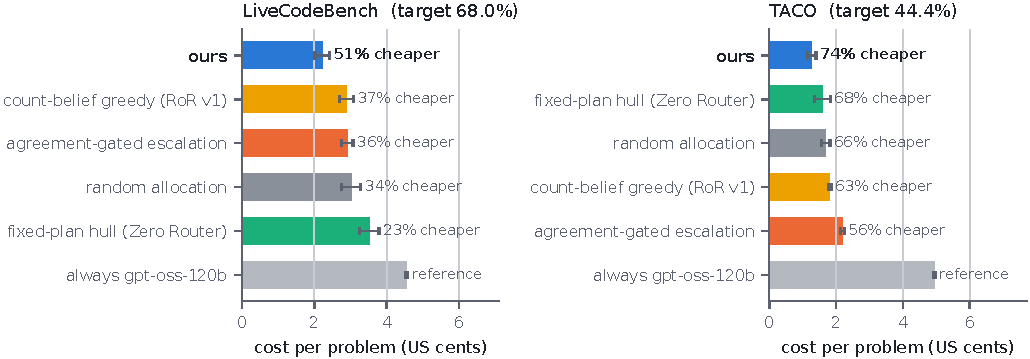
\includegraphics[width=\linewidth]{figures/fig_anchor.pdf}
\caption{Mean cost per problem at which each policy family reaches the accuracy of calling
gpt-oss-120b on every problem (LiveCodeBench 68.0\%, TACO 44.4\%), read off each family's
convex hull under realised-cost accounting.  Error bars are standard deviations over seeds (five
on LiveCodeBench, three on TACO); labels give the saving relative to calling gpt-oss-120b.}
\label{fig:anchor}
\end{figure}

\begin{figure}[t]
\centering
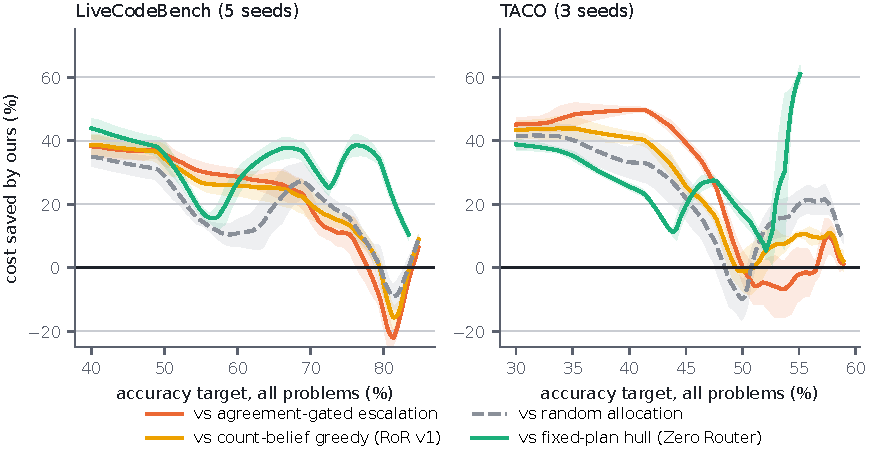
\includegraphics[width=\linewidth]{figures/fig_savings.pdf}
\caption{Cost saved by our method at matched overall accuracy, $S(\alpha)$, against each
baseline, at every accuracy both families reach on every seed.  Lines are means over seeds and
bands one standard deviation.  Positive values mean our method is cheaper.}
\label{fig:savings}
\end{figure}

Figure~\ref{fig:anchor} states the result at one operating point: reaching gpt-oss-120b's own
accuracy on LiveCodeBench costs our policy \$0.0222 per problem, 51\% less than calling
gpt-oss-120b on everything and 23\% less than the next-cheapest baseline.  On TACO the same
comparison gives 74\% and 20\%.  Figure~\ref{fig:savings} shows the saving at every reachable
target, and Table~\ref{tab:baselines} at the quoted ones.

\begin{table}[t]
\centering
\small
\caption{Cost saved at matched overall accuracy by our method against each baseline, mean
$\pm$ standard deviation over seeds, with the number of seeds on which the saving is positive.
All arms are charged realised costs.  n/a: the baseline cannot reach the target.}
\label{tab:baselines}
\begin{tabular}{lcccccc}
\toprule
\multicolumn{7}{l}{\textbf{LiveCodeBench} (5 seeds)} \\
baseline & 50\% & 60\% & 70\% & 75\% & 80\% & 84\% \\
\midrule
agreement-gated escalation & $+35.8\pm3.7$ & $+28.7\pm2.5$ & $+19.0\pm4.7$ & $+10.8\pm5.3$ & $-14.2\pm5.5$ & $+0.7\pm0.6$ \\
 & 5/5 & 5/5 & 5/5 & 5/5 & 0/5 & 5/5 \\
count-belief greedy \citep{chen2026ror} & $+34.4\pm4.2$ & $+25.9\pm3.5$ & $+20.0\pm4.6$ & $+13.8\pm2.8$ & $-5.3\pm3.9$ & $+3.7\pm1.2$ \\
 & 5/5 & 5/5 & 5/5 & 5/5 & 1/5 & 5/5 \\
random allocation & $+28.9\pm4.2$ & $+10.9\pm4.3$ & $+25.1\pm4.6$ & $+16.2\pm2.9$ & $-3.2\pm5.8$ & $+4.0\pm2.2$ \\
budget-aware best-of-$K$ & $+63.3\pm1.5$ & $+45.7\pm1.5$ & $+31.3\pm2.9$ & $+26.2\pm4.3$ & $+25.2\pm3.7$ & n/a \\
fixed-plan hull & $+35.8\pm3.8$ & $+26.9\pm4.3$ & $+33.0\pm2.9$ & $+36.4\pm2.6$ & $+30.3\pm3.1$ & n/a \\
\midrule
\multicolumn{7}{l}{\textbf{TACO} (3 seeds)} \\
baseline & 35\% & 40\% & 45\% & 50\% & 55\% & \\
\midrule
agreement-gated escalation & $+48.2\pm3.7$ & $+49.7\pm1.1$ & $+39.3\pm1.7$ & $+0.4\pm5.1$ & $-2.1\pm8.3$ & \\
 & 3/3 & 3/3 & 3/3 & 2/3 & 2/3 & \\
count-belief greedy \citep{chen2026ror} & $+43.9\pm3.6$ & $+41.0\pm1.9$ & $+25.6\pm2.2$ & $-1.2\pm6.2$ & $+10.5\pm1.0$ & \\
 & 3/3 & 3/3 & 3/3 & 1/3 & 3/3 & \\
random allocation & $+40.3\pm4.6$ & $+33.2\pm4.9$ & $+21.9\pm6.8$ & $-10.4\pm6.8$ & $+20.0\pm4.2$ & \\
budget-aware best-of-$K$ & $+64.7\pm0.6$ & $+61.0\pm0.6$ & $+49.4\pm1.0$ & $+12.6\pm7.2$ & $+39.9\pm5.4$ & \\
fixed-plan hull & $+35.3\pm1.4$ & $+25.6\pm1.1$ & $+19.6\pm2.8$ & $+17.0\pm2.6$ & $+60.2\pm2.5$ & \\
\bottomrule
\end{tabular}
\end{table}

Three patterns hold across both pools.  First, the saving is largest when money is tight: at
the lowest targets our policy is 29--50\% cheaper than every adaptive baseline on every seed,
because it declines problems it predicts it will not solve instead of paying to discover that.
Second, the adaptive baselines are close to each other, and random allocation is competitive
with the two informed ones; neither agreement nor pool-level beliefs carries much per-problem
information.  Third, the saving is not uniform in the target.  On LiveCodeBench our policy is
more expensive than the adaptive baselines between about 78\% and 83.5\% accuracy (by up to 21\%
against agreement-gated escalation near 81\%), and on TACO it ties agreement-gated escalation
near 50\%.  These bands sit just below each pool's ceiling (84.8\% and 58.9\%), where every
policy attempts almost every problem and the remaining decision is which of the hard problems
to keep paying for --- the regime in which our beliefs are weakest
(Section~\ref{sec:diagnostics}).

\subsection{The belief source is what pays}
\label{sec:isolation}

\begin{figure}[t]
\centering
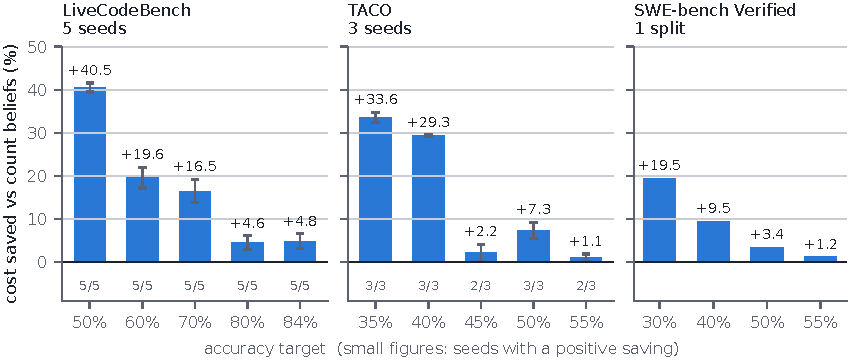
\includegraphics[width=\linewidth]{figures/fig_isolation.pdf}
\caption{Cost saved at matched accuracy by prefill beliefs over count beliefs with everything
else fixed: the same decision rule and give-up action, and the same constant per-route costs on
both sides.  LiveCodeBench and TACO: mean $\pm$ standard deviation over seeds, with the number
of seeds on which the saving is positive.  SWE-bench Verified: a single split.}
\label{fig:isolation}
\end{figure}

To isolate the belief source we compare our rule with prefill beliefs against the same rule with
count beliefs, with constant per-route costs on both sides so that the cost head plays no part.
The saving is positive at all 14 targets on three pools (Figure~\ref{fig:isolation}), and on
every seed at 8 of the 10 seeded targets (the exceptions are two TACO targets, positive on 2 of 3
seeds).  On
LiveCodeBench it is $+40.5\pm1.0\%$ at the 50\% target and $+4.8\pm1.7\%$ at 84\%; on TACO,
$+33.6\pm1.1\%$ at 35\%; on SWE-bench Verified, a different task family with five API models,
$+19.5\%$ at 30\%.

\paragraph{Which beliefs.}
Figure~\ref{fig:ladder} varies only the belief source on LiveCodeBench (one seed; same rule,
constant costs, identical fitting protocol).  Prompt length recovers almost nothing of what
perfect beliefs would save.  TF-IDF of the problem statement recovers 16--17\% at two targets
and nothing at the third.  A $k$-nearest-neighbour estimate on the same activations, and a
scorer that learns a per-problem decay constant, recover less than the linear probe, which
recovers 54\%, 27\% and 17\% at the 50\%, 60\% and 70\% targets.  As a standalone difficulty
predictor, under the same estimator and penalty grid, the probe also beats the text baselines
at predicting whether any model in the pool solves a problem (test AUC 0.824 vs.\ 0.729 for
TF-IDF on LiveCodeBench, 0.885 vs.\ 0.746 on TACO), and beats TF-IDF on per-query cost $R^2$ for
all six route--pool pairs, by 0.12 to 0.42.

\begin{figure}[t]
\centering
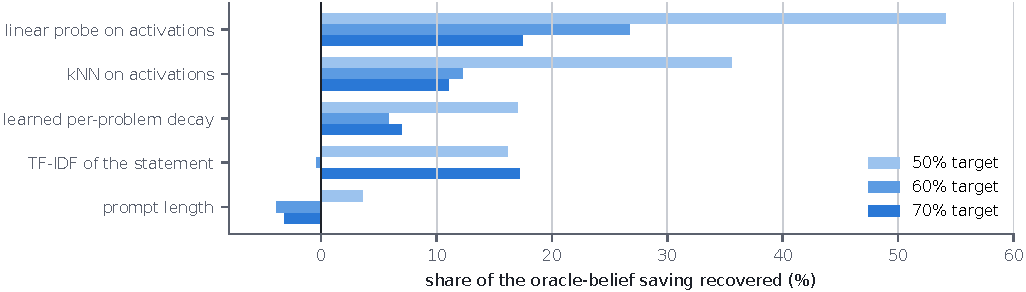
\includegraphics[width=\linewidth]{figures/fig_ladder.pdf}
\caption{Share of the oracle-belief saving recovered by each belief source (LiveCodeBench, one
seed, constant costs, identical rule).  The oracle uses each problem's empirical solve rates as
beliefs and saves 75\%, 72\% and 69\% over count beliefs at the three targets.}
\label{fig:ladder}
\end{figure}

\subsection{Where the savings come from}
\label{sec:mechanism}

Our method differs from the count-belief greedy baseline in two ways: where the beliefs come from,
and how spend is controlled (a price with a give-up action, against a cap with none).
Table~\ref{tab:twobytwo} crosses the two, with constant costs throughout.

\begin{table}[t]
\centering
\small
\caption{Beliefs crossed with budget control, with constant per-route costs on every arm.  Each
row changes one component; positive values mean the changed arm is cheaper at matched accuracy.
Mean over seeds (5 on LiveCodeBench, 3 on TACO); $^\dagger$ marks entries whose sign is not the
same on every seed.}
\label{tab:twobytwo}
\begin{tabular}{lcccc}
\toprule
\textbf{LiveCodeBench} & 50\% & 60\% & 70\% & 80\% \\
\midrule
count $\to$ prefill beliefs, price with give-up & $+40.5$ & $+19.6$ & $+16.5$ & $+4.6$ \\
count $\to$ prefill beliefs, cap without give-up & $-0.6^\dagger$ & $+13.1$ & $+7.1$ & $-0.2^\dagger$ \\
cap $\to$ price with give-up, count beliefs & $-36.2$ & $-9.4$ & $-29.3$ & $-26.4$ \\
cap $\to$ price with give-up, prefill beliefs & $+19.4$ & $-1.2^\dagger$ & $-16.2$ & $-20.5$ \\
\midrule
\textbf{TACO} & 35\% & 40\% & 45\% & 50\% \\
\midrule
count $\to$ prefill beliefs, price with give-up & $+33.6$ & $+29.3$ & $+2.2^\dagger$ & $+7.3$ \\
count $\to$ prefill beliefs, cap without give-up & $+4.8$ & $+6.4$ & $+5.4$ & $+4.8$ \\
cap $\to$ price with give-up, count beliefs & $+10.7$ & $+18.0$ & $+20.9$ & $-18.2$ \\
cap $\to$ price with give-up, prefill beliefs & $+37.7$ & $+38.0$ & $+18.3$ & $-15.3$ \\
\bottomrule
\end{tabular}
\end{table}

\paragraph{Giving up pays with per-query beliefs.}
Count beliefs are identical for every problem before the first draw, so a policy using them cannot
decline selectively; it must pay for failures before its belief falls far enough to stop.  On
LiveCodeBench, replacing the cap with a price and give-up action under count beliefs makes the
policy more expensive at every target on every seed, while with prefill beliefs the same change
saves 19\% at the tightest target.  On TACO, where 41\% of test problems are unsolved by every
draw, giving up helps even with count beliefs (by 11--21\% at three targets), and prefill beliefs
roughly double that (18--38\%).

\paragraph{Prefill beliefs pay under either control, but more with a price.}
Under a cap the prefill beliefs are worth 5--13\% at most targets; under a price they are worth
up to 41\% on LiveCodeBench and 34\% on TACO, with the largest gains at the tightest targets.

\paragraph{The cap and the price are complementary.}
With prefill beliefs, the price is the better control at tight budgets and the cap at loose ones
(last row of each block).  This is why our method sweeps both (Section~\ref{sec:cap}).  Adding
the cap to the price-only policy lowers cost at matched accuracy by 11--25\% between the 50\% and
75\% targets on LiveCodeBench and by 4--12\% on TACO, on every seed.

\paragraph{A price-swept policy has no version without abstention.}
Remove the give-up action and the surplus rule buys draws until success or exhaustion at every
price: on LiveCodeBench, all 35 zero-abstention operating points of the count-belief price arm
collapse to one point (\$0.173 per problem, 84.8\% accuracy), and ours to another.  A cap without
a give-up action gives a frontier; a price without one does not.
\begin{center}
\small
\begin{tabular}{lll}
\toprule
spend control & stopping action & frontier \\
\midrule
per-episode cap & none & a curve (the count-belief greedy baseline) \\
price $R$ & none & a single point \\
price $R$ & zero-value abstention & a curve (ours) \\
\bottomrule
\end{tabular}
\end{center}
The density rule of \citet{chen2026ror} needs its cap because $p_m/c_m$ never crosses zero; our
rule needs its give-up action for the same reason.  ``Our method without abstention'' is therefore
not a meaningful ablation.  The informative ablations are the rows of Table~\ref{tab:twobytwo}.

\paragraph{Most of the tight-budget value is the decision to start.}
Under a protocol in which the policy may decline before buying any draw (one seed), using
prefill beliefs only for the first decision and count beliefs afterwards saves 25.0\% at the
50\% target, against 43.3\% for prefill beliefs throughout; using them only after the first draw
saves 40.8\%.  At the 70\% target and above the entry-only policy saves at most 1\%, and the
value comes from tracking the prior through the episode.

\paragraph{The sequential structure extends the reachable range.}
With the same prefill beliefs, a policy that commits to one route for one draw saves 15.1\% at
the 50\% target and loses 10.0\% at 60\% (one seed, against count beliefs under the same rule),
and cannot reach 70\% at any price; the sequential policy saves 40.8\% and 19.2\% and reaches
84.8\%.  Resampling is what buys the high-accuracy regime.

\subsection{Selective prediction}
\label{sec:selective}

The simplest use of the probe needs no MDP.  Rank problems by the probe's predicted probability
that any model in the pool solves them, attempt the top fraction, and measure the share of
attempted problems that no model solves --- money spent on problems that cannot be solved.

\begin{center}
\small
\begin{tabular}{lcccccc}
\toprule
benchmark & $n$ & pool-unsolvable & AUC & AURC & oracle AURC & gap to oracle closed \\
\midrule
LiveCodeBench & 171 & 15.2\% & 0.759 & 0.062 & 0.013 & 64.9\% \\
TACO & 168 & 41.1\% & 0.838 & 0.185 & 0.100 & 72.7\% \\
SWE-bench Verified & 369 & 28.7\% & 0.703 & 0.182 & 0.046 & 43.8\% \\
\bottomrule
\end{tabular}
\end{center}
At 50\% coverage the share of attempts spent on unsolvable problems falls from 15.2\% to 5.8\% on
LiveCodeBench, from 41.1\% to 19.0\% on TACO and from 28.7\% to 16.3\% on SWE-bench Verified.
(On LiveCodeBench and TACO a problem counts as unsolvable if no draw of any route solves it.)

\subsection{Which tier, not which peer}
\label{sec:whethernotwhich}

The probe predicts how hard a problem is.  That supports every decision that is monotone in
difficulty: whether a problem is worth attempting and, on a pool whose models are ordered by both
price and ability, which tier to try --- cheap models for easy problems, large ones for hard
problems.  On our three-tier pool, prefill beliefs save 7--13\% at LiveCodeBench's middle targets
and 5--9\% on TACO through the choice of which draw to buy alone, with no give-up action
(Table~\ref{tab:twobytwo}, second row of each block).  What a difficulty estimate cannot support
is a choice among comparable models.

\paragraph{A pool with routing headroom.}
On the five-lab peer pool the best single model solves 71.9\% of test problems and the pool's
oracle 85.4\%, with 52.6\% of problems contested.  A router built on the probe captures none of
the gap:
\begin{center}
\small
\begin{tabular}{lcccc}
\toprule
router & accuracy & cost & accuracy per \$ & models used \\
\midrule
shared difficulty latent (2 parameters per model) & 70.2\% & \$0.0169 & 41.4 & 1 of 5 \\
latent plus 8 principal components & 70.8\% & \$0.0226 & 31.4 & 5 of 5 \\
per-model probe on activations & 64.9\% & \$0.0284 & 22.9 & 5 of 5 \\
best single model & 71.9\% & \$0.0321 & 22.4 & --- \\
oracle (cheapest model that solves) & 85.4\% & \$0.0179 & 47.7 & --- \\
\bottomrule
\end{tabular}
\end{center}
The five models' success curves are monotone in the same difficulty latent with similar slopes,
so one model dominates across the whole latent range and the router picks it for 171 of 171
problems --- the router collapse described by \citet{routingcollapse2026}.  A one-dimensional
latent can say how hard a problem is, and thresholds on it select a tier; it cannot say which of
several comparable models suits the problem, which needs the models' ordering to change from
problem to problem.  Adding dimensions lowers accuracy per dollar.  (On our tiered pool,
single-commit routing by the probe captures 22--31\% of the oracle's gain; one model dominates,
so a cheaper route that also succeeds is rare; Appendix~\ref{app:singleshot}.)

\paragraph{Shared factors are predictable; interactions are not.}
Per-model cost on the peer pool is partly predictable from the \scout's activations (dollar $R^2$
from 0.03 to 0.39 across the five models), but the cost \emph{ratio} between two models is not,
for any of the 10 pairs --- and the ratio is what model selection compares.  The structure exists:
the log-cost matrix is not rank one (its first component explains 72.1\% of variance), and the
cheapest model changes from problem to problem.  The prompt representation carries the factors
shared across the pool (this problem is hard, this problem is long) and not the model-by-problem
interaction (this model struggles with this problem).  Success decomposes the same way, which is
why abstention works and routing does not.

\paragraph{RouterBench.}
RouterBench is the opposite regime: 91.4\% of problems contested and 3.9\% unsolvable.  Using the
\scout's activations for every prompt and RouterBench's AIQ metric, the probe improves AIQ by
3.91\% over the Zero Router, against 2.43\% for TF-IDF and $-6.03\%$ for shuffled predictions.
This is a small gain, of the size RouterBench's own routers achieve \citep{hu2024routerbench},
and part of it is task identity rather than difficulty: RouterBench pools about 85 source
datasets, and 68\% of the variance in the probe's predictions lies between datasets against 15\%
of the variance in true success.  We report it as a boundary case, not as a result.

\subsection{Transfer and choice of encoder}
\label{sec:transfer}

\paragraph{New models at about 25 labels.}
A monotone link cannot change a ranking, so the probe's ordering of problems transfers to a new
model with no labels; labels buy calibration.  We fit a one-dimensional difficulty latent on the
three local routes and apply it to the five API peer models, which the probe has never seen,
fitting a two-parameter link per model from $N$ labelled problems:
\begin{center}
\small
\begin{tabular}{lcccccc}
\toprule
peer & solve rate & AUC & Brier, $N{=}10$ & $N{=}25$ & $N{=}170$ & base rate, $N{=}25$ \\
\midrule
deepseek-v4-flash & 0.702 & 0.746 & 0.2247 & 0.1902 & 0.1812 & 0.2192 \\
glm-5 & 0.620 & 0.812 & 0.2064 & 0.1986 & 0.1822 & 0.2559 \\
kimi-k2.5 & 0.719 & 0.790 & 0.1943 & 0.1794 & 0.1629 & 0.2134 \\
minimax-m2.7 & 0.544 & 0.811 & 0.2572 & 0.1986 & 0.1815 & 0.2668 \\
qwen3-max & 0.520 & 0.787 & 0.2441 & 0.2062 & 0.1925 & 0.2616 \\
\midrule
mean & & 0.789 & 0.2253 & 0.1946 & 0.1801 & 0.2434 \\
\bottomrule
\end{tabular}
\end{center}
At $N=25$ the latent beats each model's own base rate by 20\% of Brier score on average, and it
saturates quickly (0.1946, 0.1857 and 0.1801 at 25, 50 and 170 labels).  On the local pool, 25
labels through the latent beat a dedicated probe trained on 550 (test AUC 0.790 vs.\ 0.776).  The
transfer fails where the probe is weak: on SWE-bench Verified, where peer AUC is 0.62--0.67, the
new model's base rate is better calibrated at every $N$ up to 219.

\paragraph{The smallest model is the best encoder.}
Changing only the prefill model, the 4B \scout gives the highest mean test AUC over the three
routes (0.868), above gpt-oss-120b (0.862) at a 42nd of the prefill cost.  General-purpose models
beat code-specialised ones at matched scale: under one extraction protocol, Qwen3-0.6B (0.853)
beats Qwen2.5-Coder-3B (0.840) and Qwen2.5-Coder-1.5B (0.842).  A 0.69B model retains 95\% of the
4B model's AUC for pool solvability while solving almost none of the problems itself: the probe
reads a property of the problem, not of the solver.  This extends encoder--target decoupling
\citep{prefillrouter2026} to a sequential pool.

\paragraph{Prompt and free scalars.}
The \scout's system prompt asks it to solve the problem.  Replacing it with ``You are a helpful
assistant.'' raises mean test AUC from 0.867 to 0.877, and a prompt asking the model to judge
difficulty raises it to 0.869.  The AUC gain does not reach the policy: through an identical
fitting pipeline, the plain prompt's saving differs from the solving prompt's by $-0.8$, $0.0$,
$+6.7$, $-0.7$ and $+1.2$ points at the 50--84\% targets (three seeds, consistent only at 70\%).
Three scalars available from the same prefill (prompt negative log-likelihood, next-token entropy
and maximum next-token log-probability) carry signal alone (AUC 0.61--0.78) but change the
probe's AUC by at most 0.0002 when appended.

\subsection{Robustness}
\label{sec:robust}

\paragraph{Realised accounting.}
A per-episode cap checked against \emph{estimated} spend bounds planned spend only: implemented
that way, a third of the count-belief baseline's episodes exceed their cap, by up to
$22.3\times$.  Every result in this paper checks caps against realised spend, for our method and
for every baseline.

\paragraph{Charging for failures.}
Our accounting charges nothing for an abstention.  At matched overall accuracy, however, two
policies fail on the same number of problems, whether by abstaining or by returning a wrong answer
--- and with executable tests a wrong answer can be turned into a declared failure at the price of
one test run.  Any fixed charge per failure therefore adds the same amount to both policies'
costs; it shrinks every saving toward zero but cannot reverse its sign.

\paragraph{Price ratio.}
The method exploits the spread between cheap and expensive routes.  Moving only gpt-oss-120b's
price, and comparing the price-only policy with count beliefs under the same rule (one seed): at
a $3\times$ ratio to the \scout the saving at the 65\% target is $-118.9\%$, at $10\times$ it is
roughly zero, and from $25\times$ to our $40\times$ ratio it is stable at 13--15\%.  For
mixture-of-experts models the ratio depends on the accounting basis --- gpt-oss-120b is $30\times$
the \scout in total parameters and $1.3\times$ in active parameters --- so an operator should check
the ratio in the prices they pay.

\paragraph{A weak verifier.}
All results above let the policy observe hidden-test correctness.  If it instead observes the
public tests, which accept 11.0\% of incorrect draws, and is scored on the hidden tests, the
belief-source saving at the 50\% target falls from 40.8\% to 19.6\% (one seed) and the highest
reachable accuracy from 84.8\% to 62.1\%, because episodes end on false acceptances.

\paragraph{Fitted hyperparameters for both arms.}
The decay constant $\kappa$ is fitted separately for count and prefill beliefs.  Fitting it for
the baseline as well as for our method narrows our utility-level advantage on TACO (from 57 to 46
of 96 swept prices); every number in this paper uses fitted constants on both sides.

\subsection{What does not help, and where the headroom is}
\label{sec:diagnostics}

\paragraph{Deeper lookahead.}
Relative to the one-step rule, two-step lookahead is more expensive at the tightest target and
cheaper at the loosest ones (one seed); four-step, six-step and the exact 18-step solve are no
better than two-step, and the exact solve is worse at the 84\% target.  Because the one-step rule
already stops where the optimal policy stops (Section~\ref{sec:rule}), lookahead acts only on the
order of routes.  The lattice treats a failure on one route as uninformative about the others,
which over-values trying a cheap route first for the option it leaves open; the
correlated version of the problem is Pandora's box with correlations
\citep{gergatsouli2023weitzman}, and a more exact optimisation of the independent model does not
help.  Appendix~\ref{app:variants} lists five further single-seed variants of the rule.

\paragraph{A learned per-problem decay.}
A scorer that predicts a per-problem decay constant beats count beliefs at four of five targets,
and the probe beats it at four of five (by 32.1\%, 15.7\%, 7.6\% and 2.6\% at 50--80\%).

\paragraph{Selecting heads on predictor metrics.}
Four changes each improved their head's own metric and made the frontier worse: a stronger
belief penalty chosen on AUC, a cost penalty chosen on $R^2$, a cross-route coupling term in the
beliefs, and isotonic recalibration.  AUC is invariant to monotone transforms, whereas the rule
consumes the values of $p_mR-c_m$ and abstains on their sign; better-regularised heads are more
compressed, and the rule needs spread.

\paragraph{Probing every model.}
One prefill per pool member, including gpt-oss-120b, costs $48.5\times$ the \scout prefill.
Given away free, per-model probing is cheaper at five of six targets (by 0.6 to 8.6 points);
charged its price, it is more expensive at all six, by 10.9 to 38.5 points.

\paragraph{Headroom.}
Replacing one component at a time with ground truth at the 80\% and 84\% targets: perfect
beliefs would save 65.5\% and 73.4\% over count beliefs, perfect stopping 44.0\% and 65.0\%, and
perfect routing 8.3\% at 84\% (one seed).  In the same run the probe saves 2.3\% and 6.6\%, a
small fraction of what perfect beliefs would give.  This headroom is real rather than draw noise: after removing binomial
variance, 92--98\% of the between-problem variance in observed solve rates is systematic (per-route
ICC 0.975, 0.917 and 0.924).  The loose end of the frontier is a belief-quality problem --- knowing
which hard problems are hopeless --- and it is where the method is weakest.

\section{Limitations}
\label{sec:limitations}

\begin{enumerate}
\item \textbf{Sampling temperature.}  All three routes were sampled at temperature 0.2, below
the providers' recommended settings.  Lower temperature makes repeated draws more alike, which
changes the value of resampling and the signal available to agreement-gated escalation.  The
LiveCodeBench and TACO pools should be recollected at the recommended temperatures before these
numbers are taken as final.  SWE-bench Verified, RouterBench and the peer pool are single-draw
and unaffected.
\item \textbf{Pools.}  The two seeded pools are both competitive programming; SWE-bench Verified
is a single split of 369 problems, and several diagnostics (the belief ladder, entry versus
continuation, single-commit routing, lookahead, the price-ratio sweep, the weak verifier) rest
on one seed of LiveCodeBench.
\item \textbf{A band of targets where we lose.}  Just below each pool's ceiling our method is
more expensive than the adaptive baselines (Section~\ref{sec:headline}).
\item \textbf{Price ratio.}  The method needs a large price spread between routes, of order
$25\times$ on LiveCodeBench (Section~\ref{sec:robust}).
\item \textbf{Verifier.}  The main results assume the policy observes hidden-test correctness;
with public tests the gain roughly halves and the reachable accuracy falls
(Section~\ref{sec:robust}).
\item \textbf{The cost head is pool-dependent.}  On LiveCodeBench it improves the frontier; on
TACO, whose cost head has the lowest $R^2$ we measure, it is harmful at some targets, and the
choice of whether to use it should be made on the calibration split.
\item \textbf{Routing claims.}  The negative routing result rests on one pool with routing
headroom (the peer pool) and one boundary case (RouterBench) whose probe partly learns task
identity.
\end{enumerate}

\section{Conclusion}
\label{sec:conclusion}

One prefill of the cheapest model in a pool, read by two linear heads per model, is enough to run
a budgeted policy that resamples, reroutes and gives up.  Against the baselines a practitioner
would otherwise deploy, the policy reaches a given accuracy for substantially less money across
most of the accuracy range, and the saving comes from the per-query beliefs: with count beliefs
the same policy gains little or nothing from its give-up action.  The beliefs say how hard a
problem is.  That is enough to decide whether to attempt a problem and which tier of model to
try, but not which of several comparable models suits it.  They
transfer to models whose weights are never seen at the cost of a few dozen labels, and they
recover a small share of what perfect beliefs would save near the top of the accuracy range,
which is where further work on the representation would pay.

\paragraph{Reproducibility.}
All results are replays over stored outcome tensors; every number traces to a committed script
and a named run.  We release the replay harness, the pool-construction code and the probe
training pipeline.

\bibliography{tmlr}
\bibliographystyle{tmlr}

\appendix

\section{Terminology}
\label{app:terminology}

\begin{center}
\small
\begin{tabular}{lp{10.8cm}}
\toprule
term & meaning \\
\midrule
\scout & the cheapest model in the pool; its prefill is computed before any generation \\
prefill beliefs & per-route success probabilities $\hat\theta_m(x)$ from one \scout prefill \\
count beliefs & per-route training-set solve rates, decayed by observed failures only \\
give-up, abstention ($\abst$) & the zero-value action of the rule \\
$R$ & the dollar value of a correct answer; the inverse of the budget's Lagrange multiplier \\
$B$ & a per-episode cap on realised spend \\
$Q^{\pi_\abst}$ & $p_mR-c_m$: the action value of the always-abstain policy, on which our rule is greedy \\
baseline & a deployable policy with no abstention (Section~\ref{sec:arms}) \\
control & a variant of our method used for attribution; controls may abstain \\
contested & share of problems solved by more than one model \\
pool-unsolvable & share of problems solved by no model in the pool \\
hull & the upper convex hull of a family's (cost, accuracy) operating points \\
\bottomrule
\end{tabular}
\end{center}

\section{Method variants}
\label{app:variants}

Cost at matched accuracy against each variant's own control (LiveCodeBench, seed 0, matched
geometric grid).  These are single-seed results.

\begin{center}
\small
\begin{tabular}{lccccc}
\toprule
variant & 50\% & 60\% & 70\% & 80\% & 84\% \\
\midrule
exact posterior over the success count & +11.0\% & +5.7\% & +5.9\% & +0.9\% & $-6.5$\% \\
free-start protocol & +9.2\% & +2.2\% & $-1.4$\% & $-2.2$\% & $-1.4$\% \\
shrinking the stop test toward the mean & +12.1\% & +1.2\% & +0.8\% & +2.1\% & +0.3\% \\
cross-route coupling in the lattice & +8.0\% & +2.0\% & $-0.7$\% & $-3.6$\% & $-2.9$\% \\
90th-percentile cost head & +3.8\% & +1.2\% & +1.5\% & +5.5\% & +0.8\% \\
\bottomrule
\end{tabular}
\end{center}
Four of the five help most at the 50\% target and fade by 80\%: they all improve the give-up
decision at tight budgets, and the loose end is limited by belief quality instead
(Section~\ref{sec:diagnostics}).

\section{The single-commit routing view}
\label{app:singleshot}

Reported in the routing literature's units (one draw, no resampling), routing by the probe gives
a modest gain:

\begin{center}
\small
\begin{tabular}{lccc}
\toprule
policy & accuracy & cost & accuracy per \$ \\
\midrule
LiveCodeBench, always gpt-oss-120b & 68.9\% & \$0.0393 & 17.5 \\
LiveCodeBench, routed by the probe & 67.7\% & \$0.0343 & 19.8 \\
LiveCodeBench, oracle (cheapest that solves) & 72.5\% & \$0.0290 & 24.9 \\
TACO, always gpt-oss-120b & 47.6\% & \$0.0429 & 11.1 \\
TACO, routed by the probe & 48.2\% & \$0.0390 & 12.4 \\
TACO, oracle & 54.8\% & \$0.0320 & 17.1 \\
\bottomrule
\end{tabular}
\end{center}
Single-commit routing improves accuracy per dollar by 12--13\%, 22--31\% of the oracle's gain.
This pool has a dominant model, so there is rarely a cheaper route that also succeeds; routing
headroom is a property of the pool (Section~\ref{sec:whethernotwhich}).

\end{document}
